%%% LaTeX Template: Article/Thesis/etc. with colored headings and special fonts
%%%
%%% Source: http://www.howtotex.com/

\documentclass[12pt]{article}


\usepackage{apuntes-estilo}
\usepackage{fancyhdr,lastpage}


\def\maketitle{

% Titulo 
 \makeatletter
 {\color{bl} \centering \huge \sc \textbf{
 El shell o intérprete de comandos \\ 
\large \vspace*{-8pt} \color{black} Guía básica de uso del shell
 \vspace*{8pt} }\par}
 \makeatother


% Autor
 \makeatletter
 {\centering \small 
 	Departamento de Ingeniería de Computadoras \\
 	Facultad de Informática - Universidad Nacional del Comahue \\
 	\vspace{20pt} }
 \makeatother

}

% Custom headers and footers
\fancyhf{} % clear all header and footer fields
\fancypagestyle{plain}{\fancyhf{}}
  	\pagestyle{fancy}
 	\lhead{\footnotesize Aprendiendo Vim Progresivamente - Departamento de Ingeniería de Computadoras}
 	\rhead{\footnotesize \thepage\ }	% ''Page 1 of 2''

\def\ti#1#2{\texttt{#1} & #2 \\ }



\begin{document}

\thispagestyle{empty}
\maketitle
\setlength{\parindent}{0pt}



\section{Redireccionamientos}

Una vez hemos aprendido a utilizar algunos de los comandos del sistema, es muy probable que en 
algunos casos nos interese utilizarlos de manera simultánea para agilizar las 
acciones que queremos realizar. Una operación muy interesante consiste en poder 
tomar la salida de un comando para que sirva de entrada a otro y procesarla adecuadamente. 
El sistema operativo utiliza un mecanismo de pipes (tuberías), que nos permite redirigir las salidas 
de cualquier comando o programa hacia donde queramos. Su funcionamiento es muy simple: se trata de poner el 
carácter ``\textbar'' entre los comandos, de manera que la salida del primero sirve como
 entrada para el segundo.

Ejemplo: al escribir el comando 
\texttt{echo campo1:campo2:campo3:campo4}, lo único que conseguiríamos sería que por 
pantalla nos apareciera ``\texttt{campo1:campo2:campo3:campo4}''. Si de esta salida sólo 
quisiéramos tomar el  ``\texttt{campo3}'', podríamos redirigirla con un pipe hacia el 
comando cut, para que seleccione únicamente el campo que nos interesa de la siguiente manera: 
\texttt{echo campo1:campo2:campo3:campo4 | cut -d: -f 3}. 

En la siguiente figura podemos ver este ejemplo de manera gráfica:

\begin{center}
 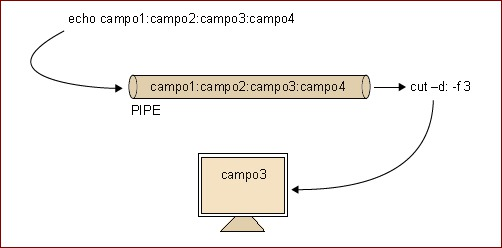
\includegraphics{./img/redireccionamiento.jpg}
 % redireccionamiento.gif: 502x248 pixel, 72dpi, 17.71x8.75 cm, bb=0 0 502 248
\end{center}


Naturalmente, podemos conectar tantas tuberías como necesitemos para realizar 
acciones más prácticas que la que acabamos de ver. Otro tipo de 
redireccionamientos muy prácticos son aquellos que están relacionados con los 
ficheros. Este tipo de redireccionamiento nos permite tomar toda la salida de 
un comando o programa y guardarla en un fichero utilizando el carácter ``\textgreater'', 
igual que hacíamos con ``\textbar''. Por ejemplo, si queremos guardar en un nuevo 
fichero todo lo que vayamos escribiendo hasta apretar ``Ctrl + C'', podríamos 
utilizar lo siguiente: \texttt{cat > prueba.txt}. Con ``\textgreater \textgreater'' 
podemos hacer exactamente 
lo mismo, pero en lugar de crear siempre el nuevo fichero, si este ya 
existiera, se añadiría la información al final del mismo. Con ``\textless'' el 
redireccionamiento se realiza en sentido contrario, de modo que el 
contenido del fichero que le indicamos se dirigirá hacia el comando o programa 
señalado.

Un aspecto muy interesante que debemos conocer es que en sistemas tipo UNIX 
se separa la salida normal de un programa con la de los errores. Aunque de  
manera predeterminada las dos salidas están dirigidas a la consola donde 
se ha ejecutado el programa, podemos manipularlas para que se dirijan hacia 
donde queramos. Para ver esto de manera práctica, intentamos borrar un fichero 
que no existe con la siguiente instrucción: \texttt{rm fichero \textgreater resultados}. Aunque 
estamos redireccionando la salida del comando hacia el fichero de resultados, 
por pantalla nos aparecerá un mensaje de error indicando que no se ha encontrado 
el fichero. Esto se debe a que de manera predeterminada los redireccionamientos sólo aceptan 
la salida estándar del programa y no la de error, que de manera predeterminada también se 
muestra por pantalla. Para redirigir la salida de error, deberíamos indicar, 
antes del carácter ``\textgreater'' el número ``2'', que es la salida de error (la ``1'' es la 
normal). De esta manera, ejecutando rm fichero 2 \textgreater resultados sí que conseguiríamos
que la salida se redirigiera al archivo de resultados. También podemos guardar 
la salida normal y la de errores en dos ficheros diferentes: rm fichero 1\textgreater resultados 2\textgreater 
errores. Si por el contrario quisiéramos que todas las salidas se dirigieran
 hacia un mismo archivo, podríamos utilizar ``\textgreater\&''. Además, con el carácter ``\&'' 
podemos encaminar salidas de un tipo hacia otras; por ejemplo, si quisiéramos 
encaminar la salida de errores hacia la normal, podríamos indicarlo del 
siguiente modo: 2\textgreater\&1.

Es importante tener en cuenta que el orden de los redireccionamiento es 
significativo: siempre se ejecutan de izquierda a derecha.

\section{Licencia}

Este material es una obra derivada de los siguientes textos:

``Sistema operativo GNU/Linux Básico'' \footnote{http://materials.cv.uoc.edu/continguts/XW07\_M2102\_02309/index.html}

© Autores: Joaquín López Sánchez-Montañés, Sofia Belles Ramos, Roger Baig i Viñas i Francesc Aulí Llinàs

© 2008, FUOC. Se garantiza permiso para copiar, distribuir y modificar este documento según los
términos de la GNU Free Documentation License, Version 1.2 o cualquiera posterior publicada por la
Free Software Foundation, sin secciones invariantes ni textos de cubierta delantera o trasera. Se dispone
de una copia de la licencia en el apartado ``GNU Free Documentation License'' de este documento.

\end{document}
